\documentclass{article}
\usepackage{graphicx} % Required for inserting 
\usepackage{amsmath,amsfonts,amssymb}
\usepackage{float}
\usepackage{tikz}
\usetikzlibrary{automata, positioning, arrows.meta, fit, shapes.geometric}
\usepackage{amsthm}
\usepackage[colorlinks=true, allcolors=blue]{hyperref}
\newtheorem{theorem}{Theorem}[section]
\newtheorem{lemma}[theorem]{Lemma}
\title{Minimal DFA's for Divisibility Testing (LSB first)}
\author{Jez Snelson \& Joshua Obayomi}
\begin{document}
\maketitle
\section{Introduction}
\section{Non-Distinguishability Criteria}
% Declare function r_b(x) at some point
% Declare distinguishability equivalence relation for divisibility by p ~_{d,p}
\subsection{Initial ND Criteria}
\begin{lemma}
  % Define notation of x = val(s_x)
  The strings $s_x,s_y$ are non distinguishable if and only if\\
  $\forall d\in\mathbb N$ $r_2(s_x)d+x\equiv0\iff r_2(s_y)d+y\equiv0$
\end{lemma}
\subsection{Revised ND Criteria}
\begin{lemma}
  For all $\alpha\in\mathbb Z/p\mathbb Z$ there exists $\alpha^{-1}\in \mathbb Z/p\mathbb Z$ if $a,p$ are coprime and $a\neq0$
\end{lemma}
\begin{proof}
If we pick $a$ and we have that $\alpha$ and $p$ are coprime we have by Bezout's identity we have that there exists integers $x$ and $y$ such that $\alpha x+py=1$ which implies that\\ 
\[\alpha x+py\equiv\alpha x+0\equiv\alpha x\equiv1\text{   (mod }p)\]\\
And so we take $\alpha^{-1}=x$ 
\end{proof}
\begin{lemma}
  \label{2.3}
 The strings $s_x,s_y$ are non distinguishable if and only if\\
 $(r_2(s_x))^{-1}x\equiv (r_2(s_y))^{-1}y \text{  (mod p)}$
\end{lemma}
\section{Equivalence Relation Classes}
As we have shown our distinguishability equivalence relation $_{d,p}$ is equivalent to $r_2(s_y)x\equiv r_2(s_x)y \text{  (mod }p)$ and we want to construct our distinguishing set from this which leads us to.\\
\begin{lemma}
  The amount of equivalence classes under $=_{d,p}$ is exactly $p$\\
  Also said as $\Sigma^*/ND=p$
\end{lemma}
\begin{proof}
  Firstly since there is only $p$ possible values for the numbers to be congruent to mod $p$ as they are integers we have that the amount of equivalence classes is $\leq p$.\\
  Now all we need to do is find $p$ possible equivalence classes of distinguishability which will force it to be $p$.\\
  Consider the strings of $0$ to $p-1$.\\
  Prepend 0s to the start of these strings to make them all the same length so we have $r_2(s_x)=\alpha$ for all of them.\\
  We then have that they are all distinct under $=_{d,p}$ as for any two such strings $s_x,s_y,x\neq y$  assuming they are non distinguishable we have by \ref{2.3} \\
  \[(r_2(s_x))^{-1}x\equiv (r_2(s_y))^{-1}y \text{  (mod p)}\]
  \[\alpha^{-1}x\equiv \alpha^{-1}y \text{  (mod p)}\]
  \[x\equiv y \text{  (mod p)}\]
  This forms a contradiction as we picked them to be distinct numbers between $0$ and $p-1$ and so they must all be distinguishable and hence in different equivalence classes.\\
  Thus we have found $p$ distinct equivalence classes and so the amount of equivalence classes is exactly $p$.
\end{proof}

\section{Even Numbers}
Now we aim to extend our Minimal DFA's to work with even numbers specifically numbers of the form $2^\alpha p$ where $\alpha,p\in\mathbb N$ and p is odd.\\
\subsection{Construction}
We will construct a proposed minimal DFA 
\subsubsection{Checking for Divisibility by 2$^\alpha$}
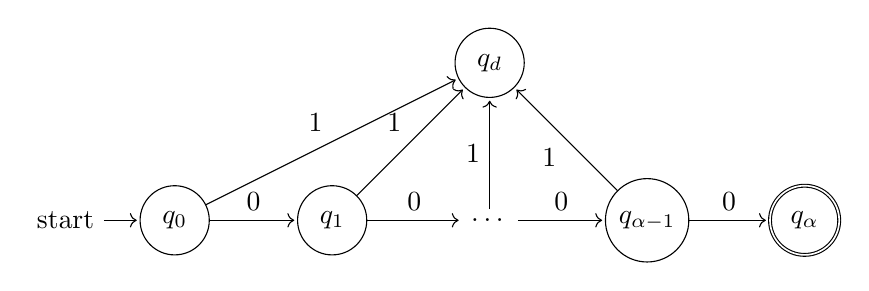
\begin{tikzpicture}[shorten >=1pt, node distance=2cm, on grid, auto]
   % First two states
   \node[state, initial] (q0) {$q_0$};
   \node[state] (q1) [right=of q0] {$q_1$};
   
   % The Dots (Ellipsis)
   \node (dots) [right=of q1] {$\dots$};
   
   % Last two states
   \node[state] (qn-1) [right=of dots] {$q_{\alpha-1}$};
   \node[state, accepting] (qn) [right=of qn-1] {$q_\alpha$};

   \node[state] (qd) [above=of dots] {$q_d$};

   % Transitions
   \path[->] 
    (q0) edge node {0} (q1)
    (q1) edge node {0} (dots)
    (dots) edge node {0} (qn-1)
    (qn-1) edge node {0} (qn)
    (q0) edge node {1} (qd)
    (q1) edge node {1} (qd)
    (dots) edge node {1} (qd)
    (qn-1) edge node {1} (qd);
\end{tikzpicture}
\\
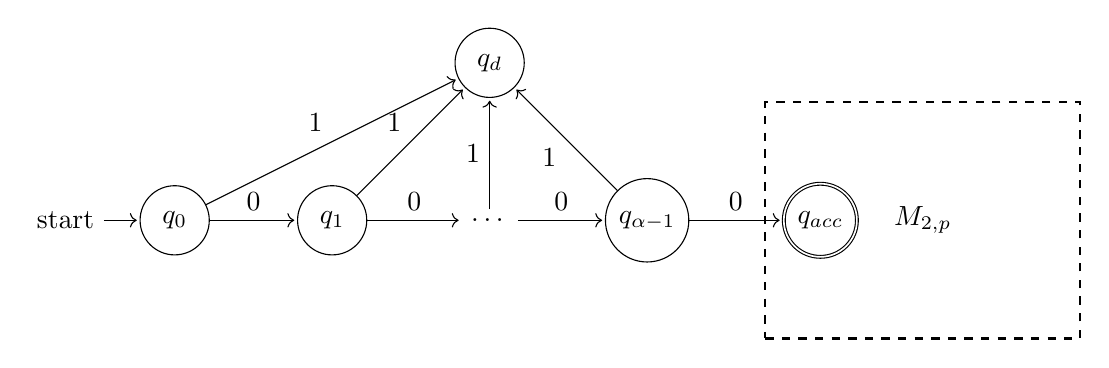
\begin{tikzpicture}[shorten >=1pt, node distance=2cm, on grid, auto]
   % First two states
   \node[state, initial] (q0) {$q_0$};
   \node[state] (q1) [right=of q0] {$q_1$};
   
   % The Dots (Ellipsis)
   \node (dots) [right=of q1] {$\dots$};
   
   % Last two states
   \node[state] (qn-1) [right=of dots] {$q_{\alpha-1}$};

   \node[state, accepting] (q_acc) [right=2.2cm of qn-1] {$q_{acc}$};
   \node[draw, dashed, minimum width=4cm, minimum height=3cm, thick] (dfa2) [right=3.5cm of qn-1] {$M_{2,p}$};

   \node[state] (qd) [above=of dots] {$q_d$};

   % Transitions
   \path[->] 
    (q0) edge node {0} (q1)
    (q1) edge node {0} (dots)
    (dots) edge node {0} (qn-1)
    (qn-1) edge node {0} (q_acc)
    (q0) edge node {1} (qd)
    (q1) edge node {1} (qd)
    (dots) edge node {1} (qd)
    (qn-1) edge node {1} (qd);
\end{tikzpicture}
\subsection{Proof of it working}
\subsection{Reachability}
% 2^\alpha to get to the start then the pick a number from the equivalence class to get to the state
\subsection{Distinguishability}
% Odd = in p machine
% Even = in 2^\alpha machine
% Prove any odd state has a string that makes it acceptable
% Odd/Even vs Dead by string that accepts them
% Even - Odd by 1 then string that accepts the state odd gets to
% Even - Even by smallest accepting string 
\begin{lemma}
  For all $S_m$ $S_n$ in the states of $M_{2,2^\alpha p}$ we have that $S_m$ is distinguishable from $S_n$
\end{lemma}
\begin{proof}
  We split $S_m$ and $S_n$ into cases based on which part of the DFA they are in we consider 3 cases for each of them being the dead state $q_d$, being any other state in the divisibility by $2^\alpha$ part $q_l, 0<l<\alpha-1$ or being any state in $M_{2,p}$.\\
  
\end{proof}

\end{document}